%
% Template for videoprojector foils according to the HZDR corporate design
% 
% (C) 2011 Alexander Grahn, HZDR, Institut fuer Sicherheitsforschung
%
% Version 20131126
%
\documentclass[
%  aspectratio=43, %default screen size (4:3); other values: 1610, 169, 149, 54, 32
%  smaller, %uncomment this to fit more text onto the slides (similar to the CD suggestions)
  intlimits %put limits of integrals above and below the integral symbol
]{beamer}

%\usepackage[ngerman]{babel}
\usepackage[UKenglish]{babel}

%my favourite packages
\usepackage[latin1]{inputenc} %type in accented characters easily, i. e. � instead of \"a 
%\usepackage{siunitx} %easy input & nice formatting of phys. quantities (number + SI unit)
%\usepackage{latexsym}
%\usepackage{amssymb}
\usepackage{media9}
%\usepackage{animate}
\usepackage{ragged2e}\RaggedRight
\usepackage{fancyvrb}
\usepackage{ifthen}

%%%%%%%%%%%%%%%%%%%%%%%%%%%%% some optional settings %%%%%%%%%%%%%%%%%%%%%%%%%%%%%%%%%%%%
%uncomment this if you want the title page text aligned flushleft; CD rules seem to
%demand this, although it looks awful
%\def\titleflushleft{}

%uncomment this if you want frame titles centred
%\def\frametitlecentered{}

%uncomment this if you don't like the wallclock
%\def\noclock{}

%uncomment this if you don't like the navigation buttons
%\def\nonavigation{}

%uncomment this if you want Arial as the main text font (very ugly),
%no matching math font, using CM-Bright for math text
%\def\arial{}

%uncomment this if you want Helvetica as the main text font (very ugly),
%Helvetica is very similar to Arial; again, no matching math font, using CM-Bright for
%math text
%\def\helvetica{}

%hzdr colours used for various text highlights; see manual `beameruserguide.pdf',
%chapter 12 for further possibilities
                                               %colour will be used in:
\setbeamercolor{alerted text}{fg=hzdr-orange}  %\alert{text to be highlighted},
                                               %\begin{alertenv} ... \end{alertenv}
                                               %\begin{alertblock}{block title (highlighted)}
                                               %  ...
                                               %\end{alertblock}

\setbeamercolor{example text}{fg=hzdr-darkblue}%\begin{exampleblock}{block title (highlighted)}
                                               %  ...
                                               %\end{exampleblock}
%%%%%%%%%%%%%%%%%%%%%%%%%%%%%%%%%%%%%%%%%%%%%%%%%%%%%%%%%%%%%%%%%%%%%%%%%%%%%%%%%%%%%%%%%

%hzdr theme
\makeatletter
\def\input@path{{beamerthemehzdr/}}
\makeatother
\usetheme{hzdr}

%%%%%%%%%%%% title, author, date, institute, additional logos %%%%%%%%%%%%%%%%%%%%%%%%%%%
\title{HASEonGPU}
\subtitle{An Open-Source ASE code for calculating the gain in high power laser media on GPU clusters}% may be left empty, of course

%[short version of authors to be used in footlines]{long version in the title page}
\author[C. Eckert, E. Zenker et al.]{
\texorpdfstring{\underline{Carlchristian Eckert}\inst{1}}{},
\texorpdfstring{\underline{Erik Zenker}\inst{1}}{}
}


%\date{\today}
\date{15th July 2014}

\institute[
 %short version of main authors' institute, used in the footline
 \iflanguage{ngerman}{%
   Institut f�r Strahlenphysik%
 }{%
   Institute of Radiation Physics%
 }%
]{%
 %used in the title page
 \iflanguage{ngerman}{%
   \inst{1}Helmholtz-Zentrum Dresden-Rossendorf, Institut f�r Strahlenphysik\\
 }{%
   \inst{1}Helmholtz-Zentrum Dresden-Rossendorf, Institute of Radiation Physics\\
 }%
}

%every invocation of the macro \partnerlogo{...} adds YET ANOTHER partner logo to the
%right of the already inserted partner logos;
%the starred version `\partnerlogo*{}' inserts s-t-r-e-t-c-h-a-b-l-e space between the current
%logo and the next one on its right side: this allows for logos/groups of logos to be
%aligned flush-left on the page
%\partnerlogo{\colorbox{gray}{\tiny Logo 1}}% some logo
%\partnerlogo*{\colorbox{gray}{\tiny Logo 2}}% another logo with stretchable space on its right
\partnerlogo{% DD-concept logo; note that different versions are used on title and normal slides
  \ifthenelse{\theframenumber=0}{%  %title slide
    \includegraphics[height=0.08\paperheight]{DDC-weisse-schrift}%
  }{%                               %normal slides
    
\includegraphics[height=0.05\paperheight]{DDC-orig}%
  }%
}
%%%%%%%%%%%%%%%%%%%%%%%%%%%%%%%%%%%%%%%%%%%%%%%%%%%%%%%%%%%%%%%%%%%%%%%%%%%%%%%%%%%%%%%%%%

\hypersetup{%
  breaklinks,colorlinks,
  %pdfpagemode=FullScreen,
  pdfhighlight=/P,
  linkcolor=hzdr-darkblue,
  linkcolor=hzdr-darkblue,
  anchorcolor=hzdr-darkblue,
  citecolor=hzdr-darkblue,
  filecolor=hzdr-darkblue,
  menucolor=hzdr-darkblue,
  runcolor=hzdr-darkblue,
  urlcolor=hzdr-darkblue
}

\begin{document}

\frame{\titlepage}

%\noautobookmark %don't add frame titles as bookmarks to the `Bookmarks' tab of Adobe Reader

\autobookmark

\begin{frame}{ASE is a fundamental process in laser physics}
  \begin{columns}[T]

    \begin{column}{.5\textwidth}
      \textbf{graphic: ASE crystal, with a photon travelling through it?}\\[2ex]
      \textbf{alternative: laser setup, pumping a gain medium?}
    \end{column}

    \begin{column}{.5\textwidth}
      \begin{itemize}
      \myuncover{1}{3}{
        \item In laser physics, gain media are pumped by lasers\\[1ex]
      }
      \myuncover{2}{3}{
        \item Over time, electrons fall back into lower energy levels, causing
          the spontaneous emission of a photon\\[1ex]
      }
      \myuncover{3}{3}{
        \item Photon travels through the medium, where it is amplified by more
          photons that are released
      }
  \end{itemize}
    \end{column}

  \end{columns}
\end{frame}


\begin{frame}[allowframebreaks=0.8]{Pitfalls}
  \begin{itemize}
    \item The packages Beamer-3.10 and PGF-2.10 are required. Update your \TeX{}
      installation if necessary.
    \item The template works only with pdf\LaTeX{}. Therefore, graphics files
      for inclusion should be provided in the PDF format for all kinds of
      graphics (line graphics, bitmapped images, photographs), PNG for
      artificially created bitmapped material and photographs, JPEG for
      photographs. Existing EPS files can be converted to PDF using {\tt
      epstopdf}, which should be part of every \TeX{} installation.
    \item This template uses \alert{CM-Bright} as the main text font. It looks
      good and, unlike CM-Sans which Beamer uses by default, it comes with a
      suitable math font. Make sure that CM-Bright is installed as Type-1 font
      in your \TeX{} system. For this, you need the packages `cm-super' and
      `hfbright' (use the package manager of your \TeX{} system for
      installation). Otherwise, the bitmapped version of the font is used and
      the final PDF is of bad quality.
    \item If you want Arial or Helvetica, as recommended by the corporate design
      guidelines, you can adjust this in the header of the source file of this
      document. As both fonts lack a matching math font, the template uses
      CM-Bright for the glyphs in math mode. For Arial you need the `arial' and
      for Helvetica the `helvet' \LaTeX{} packages. Package `hfbright' is needed
      for the math glyphs.
  \end{itemize}
\end{frame}


\autobookmark
\begin{frame}{A fast simulation will enable new use cases}
  \begin{columns}[T]

    \begin{column}{.3\textwidth}
      \textbf{graphic: cycle between ASE calculation and it's temperature influence}
    \end{column}

    \begin{column}{.7\textwidth}
      \begin{itemize}
          \myuncover{1}{3}{
          \item ASE influences temperature of the gain medium\\[1ex]
          }
          \myuncover{2}{3}{
          \item The change in temperature creates mechanical and optical
            changes, which influence the behaviour of the medium\\[1ex]
          }
          \myuncover{3}{3}{
          \item This calculation is iterative, takes a long time. Only practival for very simplified models
          }
      \end{itemize}
    \end{column}

  \end{columns}
\end{frame}

\autobookmark
\begin{frame}[t]{ASE can be modeled as multidimensional integral}
  \begin{columns}[T]
    \begin{column}{.5\textwidth}
      \myonly{1}{\includegraphics[height=0.55\paperheight]{graphics/monte_carlo_description_0.pdf}}
      \myonly{2}{\includegraphics[height=0.55\paperheight]{graphics/monte_carlo_description_1.pdf}}
      \myonly{3}{\includegraphics[height=0.55\paperheight]{graphics/monte_carlo_description_2.pdf}}
    \end{column}
    \begin{column}{.5\textwidth}
      \begin{itemize}
        \myuncover{1}{3}{
          \item Monte Carlo integration is one way to solve this integral
        }

        \myuncover{2}{3}{
          \item Create a statistical relevant amount of photons
        }
        \myuncover{3}{3}{
          \item Amplification of these photons can be simulated with ray tracing
        }
      \end{itemize}
    \end{column}
  \end{columns}
      \myonly{3}{\[ASE(sample~point)~=~\frac{1}{N}\sum_{i=1}^N amplification(photon_i)\]}
\end{frame}

\autobookmark
\begin{frame}[t]{Monte Carlo can be implemented with ray tracing}
  \myonly{1}{\includegraphics[height=0.6\paperheight]{graphics/monte_carlo_description_2.pdf}}
  \myonly{2}{\includegraphics[height=0.6\paperheight]{graphics/monte_carlo_description_3.pdf}}
  \myonly{3}{\includegraphics[height=0.6\paperheight]{graphics/monte_carlo_description_4.pdf}}
%
%  \begin{columns}[T]
%
%    \begin{column}{.5\textwidth}
%      \textbf{graphic: ASE crystal, with a photon travelling through it?}\\[2ex]
%      \textbf{alternative: laser setup, pumping a gain medium?}
%    \end{column}
%
%    \begin{column}{.5\textwidth}
%      \begin{itemize}
%      \myuncover{1}{3}{
%        \item In laser physics, gain media are pumped by lasers\\[1ex]
%      }
%      \myuncover{2}{3}{
%        \item Over time, electrons fall back into lower energy levels, causing
%          the spontaneous emission of a photon\\[1ex]
%      }
%      \myuncover{3}{3}{
%        \item Photon travels through the medium, where it is amplified by more
%          photons that are released
%      }
%  \end{itemize}
%    \end{column}
%
%  \end{columns}
\end{frame}

\autobookmark
\begin{frame}[t]{When is the simulation precise enough?}
  \begin{columns}[T]
    \begin{column}{.5\textwidth}
       \includegraphics[width=.37\paperwidth]{graphics/gain_medium_mse.pdf}
    \end{column}

    \begin{column}{.5\textwidth}
      \begin{itemize}
        \myuncover{1}{2}{
          \item Certain areas of the gain medium produce a higher variance in amplification
          \item \textcolor{hzdr-struct}{Mean Squared Error} is used to estimate simulation quality for each sample point
        }
        \myuncover{2}{2}{
          \item Calculation is successful, when MSE is low enough for each sample point
        }

      \end{itemize}
    \end{column}
  \end{columns}
\end{frame}

%\begin{frame}{Predefined colours}
%  The template defines a set of colours according to the CD guidelines:\par
%  \begin{itemize}
%      \begin{minipage}[t]{0.5\linewidth}
%      \item \textcolor{hzdr-blue}{Helmholtz Blue}    
%      \item \textcolor{hzdr-orange}{Rossendorf Orange}  
%      \item \textcolor{hzdr-darkblue}{Helmholtz Dark Blue}
%      \item \textcolor{hzdr-gray1}{Gray1}   
%      \item \textcolor{hzdr-gray2}{Gray2}   
%      \item \textcolor{hzdr-gray3}{Gray3}   
%      \item \textcolor{hzdr-struct}{Structure of Matter}  
%      \end{minipage}%
%      \begin{minipage}[t]{0.5\linewidth}
%      \item \textcolor{hzdr-health}{Health}  
%      \item \textcolor{hzdr-energy}{Energy}  
%      \item \textcolor{hzdr-earth}{Earth and Environment}   
%      \item \textcolor{hzdr-keytec}{Key Technologies}  
%      \item \textcolor{hzdr-aero}{Aeronautics, Space and Transport}
%      \end{minipage}
%  \end{itemize}
%\end{frame}


\autobookmark
\begin{frame}{Monte Carlo ray tracing is fast on GPGPUs}
  \begin{columns}[T]

    \begin{column}{.7\textwidth}
      \begin{itemize}
          \myuncover{1}{3}{
          \item Because the elements in Monte Carlo are independent, they are
            great to be used with accelerators
          }
          \myuncover{2}{3}{
          \item We used CUDA to improve an exisiting sequential ASE code that
            used MC and ray tracing
          }
          \myuncover{3}{3}{
          \item The calculation can be distributed even more, to utilize a whole
            CPU cluster, which allows to solve huge simulations fast.
          }
      \end{itemize}
    \end{column}

    \begin{column}{.3\textwidth}
      \textbf{graphic: Nvidia CUDA logo}
    \end{column}

  \end{columns}

\end{frame}

%\begin{frame}{Predefined colours}
%  The template defines a set of colours according to the CD guidelines:\par
%  \begin{itemize}
%      \begin{minipage}[t]{0.5\linewidth}
%      \item \textcolor{hzdr-blue}{Helmholtz Blue}    
%      \item \textcolor{hzdr-orange}{Rossendorf Orange}  
%      \item \textcolor{hzdr-darkblue}{Helmholtz Dark Blue}
%      \item \textcolor{hzdr-gray1}{Gray1}   
%      \item \textcolor{hzdr-gray2}{Gray2}   
%      \item \textcolor{hzdr-gray3}{Gray3}   
%      \item \textcolor{hzdr-struct}{Structure of Matter}  
%      \end{minipage}%
%      \begin{minipage}[t]{0.5\linewidth}
%      \item \textcolor{hzdr-health}{Health}  
%      \item \textcolor{hzdr-energy}{Energy}  
%      \item \textcolor{hzdr-earth}{Earth and Environment}   
%      \item \textcolor{hzdr-keytec}{Key Technologies}  
%      \item \textcolor{hzdr-aero}{Aeronautics, Space and Transport}
%      \end{minipage}
%  \end{itemize}
%\end{frame}


\autobookmark
\begin{frame}{Distribution of rays on a GPU}
  \begin{columns}[T]

    \begin{column}{.4\textwidth}
      \includegraphics[width=0.4\paperwidth]{graphics/kernel_detail5.png}
    \end{column}

    \begin{column}{.6\textwidth}
      \begin{itemize}
          \myuncover{1}{4}{
          \item A CUDA thread proceses multiple rays
          \item Reduction over all threads by atomicAdd is the only synchronized part
          }
          \myuncover{2}{4}{
          \item Rays starting in similar positions are grouped together to improve caching
          }
          \myuncover{3}{4}{
          \item Importance sampling distributes rays in the material towards areas of interest
          }
          \myuncover{4}{4}{
          \item Load balancing between blocks, to reduce impact of different ray lengths
          }
      \end{itemize}
    \end{column}


  \end{columns}

\end{frame}

%\begin{frame}{Predefined colours}
%  The template defines a set of colours according to the CD guidelines:\par
%  \begin{itemize}
%      \begin{minipage}[t]{0.5\linewidth}
%      \item \textcolor{hzdr-blue}{Helmholtz Blue}    
%      \item \textcolor{hzdr-orange}{Rossendorf Orange}  
%      \item \textcolor{hzdr-darkblue}{Helmholtz Dark Blue}
%      \item \textcolor{hzdr-gray1}{Gray1}   
%      \item \textcolor{hzdr-gray2}{Gray2}   
%      \item \textcolor{hzdr-gray3}{Gray3}   
%      \item \textcolor{hzdr-struct}{Structure of Matter}  
%      \end{minipage}%
%      \begin{minipage}[t]{0.5\linewidth}
%      \item \textcolor{hzdr-health}{Health}  
%      \item \textcolor{hzdr-energy}{Energy}  
%      \item \textcolor{hzdr-earth}{Earth and Environment}   
%      \item \textcolor{hzdr-keytec}{Key Technologies}  
%      \item \textcolor{hzdr-aero}{Aeronautics, Space and Transport}
%      \end{minipage}
%  \end{itemize}
%\end{frame}


\autobookmark
\begin{frame}[t]{Importance sampling to counter high MSE values}
      \myonly{1}{\includegraphics[width=.37\paperwidth]{graphics/ray_distributions2.png}}
      \myonly{2}{\includegraphics[width=.37\paperwidth]{graphics/ray_distributions3.png}}
      \myonly{1}{\includegraphics[width=.5\paperwidth]{graphics/mse_histogram_uniform_is1.pdf}}
      \myonly{2}{\includegraphics[width=.5\paperwidth]{graphics/mse_histogram_uniform_is2.pdf}}
      \begin{itemize}
        \myuncover{1}{2}{
        \item Uniform distribution of photons produces high MSE
        }
        \myuncover{2}{2}{
        \item Importance sampling is used to focus on areas with high influence on the result
        }
      \end{itemize}
\end{frame}

\autobookmark
\begin{frame}[t]{Adaptive sampling to counter high MSE values}
      \myonly{1}{\includegraphics[width=.37\paperwidth]{graphics/ray_distributions3.png}}
      \myonly{2}{\includegraphics[width=.37\paperwidth]{graphics/ray_distributions4.png}}
      \myonly{1}{\includegraphics[width=.5\paperwidth]{graphics/mse_histogram_is_as1.pdf}}
      \myonly{2}{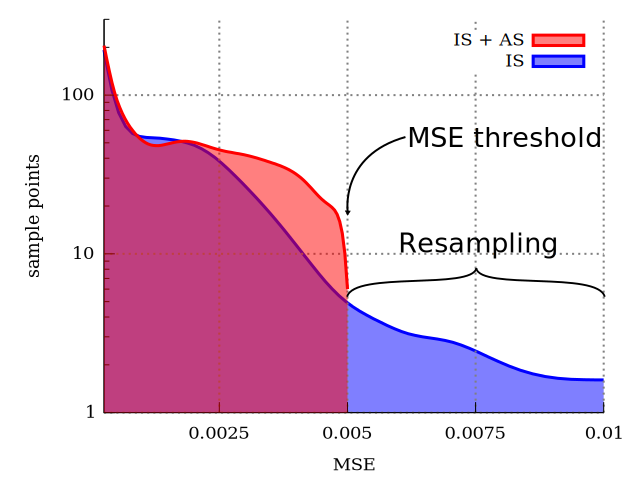
\includegraphics[width=.5\paperwidth]{graphics/mse_histogram_is_as2.pdf}}
      \begin{itemize}
        \myuncover{1}{2}{
        \item Even with importance sampling, high MSE peaks are possible
        }
        \myuncover{2}{2}{
        \item To reach a fixed MSE threshold, the number of rays for the sample point is increased
        }
      \end{itemize}
\end{frame}

\autobookmark
\begin{frame}{Restarting the simulation to counter high MSE values}
  \begin{columns}[T]

    \begin{column}{.5\textwidth}
      \includegraphics[height=0.35\paperheight]{graphics/PAP_step4_2.png}
      \myuncover{3}{3}{
        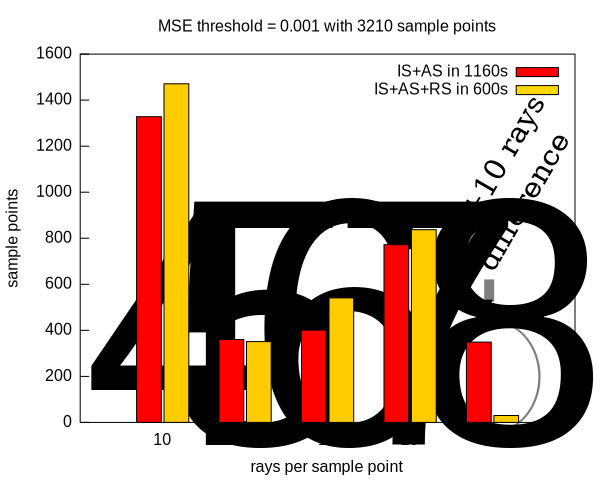
\includegraphics[height=0.35\paperheight]{graphics/repetitive_sampling.png}
      }
    \end{column}

    \begin{column}{.5\textwidth}
      \begin{itemize}
          \myuncover{1}{3}{
            \item Sometimes, increasing the number of rays is not necessary, because the high MSE was caused by a really unlucky seed for the PRNG
          }
          \myuncover{2}{3}{
            \item Idea: it might be enough to introduce random restarts, since this is much faster than increasing the number of rays
          }
      \end{itemize}
    \end{column}


  \end{columns}
\end{frame}

%\begin{frame}{Predefined colours}
%  The template defines a set of colours according to the CD guidelines:\par
%  \begin{itemize}
%      \begin{minipage}[t]{0.5\linewidth}
%      \item \textcolor{hzdr-blue}{Helmholtz Blue}    
%      \item \textcolor{hzdr-orange}{Rossendorf Orange}  
%      \item \textcolor{hzdr-darkblue}{Helmholtz Dark Blue}
%      \item \textcolor{hzdr-gray1}{Gray1}   
%      \item \textcolor{hzdr-gray2}{Gray2}   
%      \item \textcolor{hzdr-gray3}{Gray3}   
%      \item \textcolor{hzdr-struct}{Structure of Matter}  
%      \end{minipage}%
%      \begin{minipage}[t]{0.5\linewidth}
%      \item \textcolor{hzdr-health}{Health}  
%      \item \textcolor{hzdr-energy}{Energy}  
%      \item \textcolor{hzdr-earth}{Earth and Environment}   
%      \item \textcolor{hzdr-keytec}{Key Technologies}  
%      \item \textcolor{hzdr-aero}{Aeronautics, Space and Transport}
%      \end{minipage}
%  \end{itemize}
%\end{frame}


\autobookmark
\begin{frame}{Sample points can be distributed in a cluster}
  \begin{columns}[T]

    \begin{column}{.4\textwidth}
      \myuncover{3}{4}{
      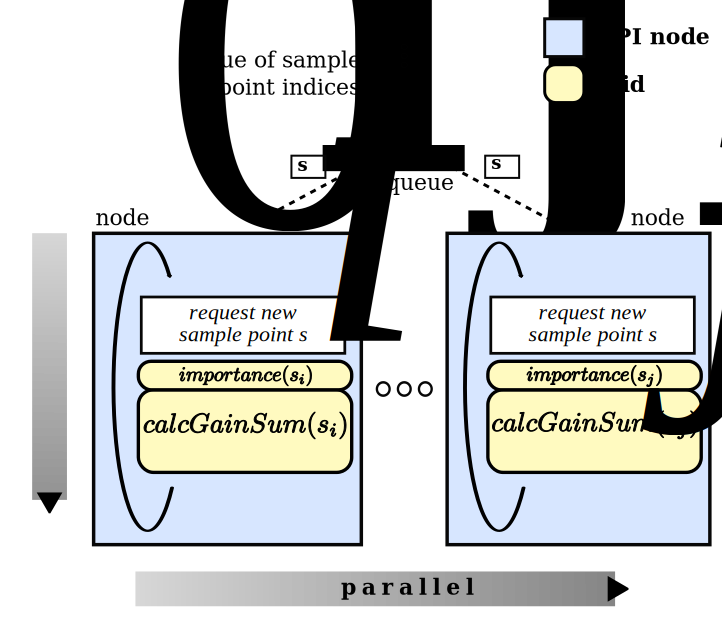
\includegraphics[width=0.4\paperwidth]{graphics/multigpu_partitioning5.png}
    }
    \end{column}

    \begin{column}{.6\textwidth}
      \begin{itemize}
          \myuncover{1}{4}{
            \item Until now: simulation of a single sample point on a single GPU
            \item All sample points are independent: let's use a cluster for that
          }
          \myuncover{2}{4}{
            \item Each GPU has all the necessary data
            \item MPI is used as communication framework
          }
          \myuncover{3}{4}{
            \item Compute nodes request work from head node
            \item Head node tells each worker, which sample point to simulate next
          }
          \myuncover{4}{4}{
            \item Load balancing, even when some sample points take longer than others
          }
      \end{itemize}
    \end{column}

  \end{columns}
\end{frame}

%\begin{frame}{Predefined colours}
%  The template defines a set of colours according to the CD guidelines:\par
%  \begin{itemize}
%      \begin{minipage}[t]{0.5\linewidth}
%      \item \textcolor{hzdr-blue}{Helmholtz Blue}    
%      \item \textcolor{hzdr-orange}{Rossendorf Orange}  
%      \item \textcolor{hzdr-darkblue}{Helmholtz Dark Blue}
%      \item \textcolor{hzdr-gray1}{Gray1}   
%      \item \textcolor{hzdr-gray2}{Gray2}   
%      \item \textcolor{hzdr-gray3}{Gray3}   
%      \item \textcolor{hzdr-struct}{Structure of Matter}  
%      \end{minipage}%
%      \begin{minipage}[t]{0.5\linewidth}
%      \item \textcolor{hzdr-health}{Health}  
%      \item \textcolor{hzdr-energy}{Energy}  
%      \item \textcolor{hzdr-earth}{Earth and Environment}   
%      \item \textcolor{hzdr-keytec}{Key Technologies}  
%      \item \textcolor{hzdr-aero}{Aeronautics, Space and Transport}
%      \end{minipage}
%  \end{itemize}
%\end{frame}


\autobookmark
\begin{frame}{Implementation is scalable on cluster systems}
  \begin{columns}

    \begin{column}{.5\textwidth}
        \includegraphics[width=.5\paperwidth]{graphics/scaling.png}
      \end{column}

      \begin{column}{.5\textwidth}
        \begin{itemize}
            \item Implementation scales almost perfectly with an increasing
              number of GPUs in a cluster system
            \item It is possible to simulate even large gain media with high
              precision in a reasonable amount of time
        \end{itemize}
      \end{column}

    \end{columns}
\end{frame}

%\begin{frame}{Predefined colours}
%  The template defines a set of colours according to the CD guidelines:\par
%  \begin{itemize}
%      \begin{minipage}[t]{0.5\linewidth}
%      \item \textcolor{hzdr-blue}{Helmholtz Blue}    
%      \item \textcolor{hzdr-orange}{Rossendorf Orange}  
%      \item \textcolor{hzdr-darkblue}{Helmholtz Dark Blue}
%      \item \textcolor{hzdr-gray1}{Gray1}   
%      \item \textcolor{hzdr-gray2}{Gray2}   
%      \item \textcolor{hzdr-gray3}{Gray3}   
%      \item \textcolor{hzdr-struct}{Structure of Matter}  
%      \end{minipage}%
%      \begin{minipage}[t]{0.5\linewidth}
%      \item \textcolor{hzdr-health}{Health}  
%      \item \textcolor{hzdr-energy}{Energy}  
%      \item \textcolor{hzdr-earth}{Earth and Environment}   
%      \item \textcolor{hzdr-keytec}{Key Technologies}  
%      \item \textcolor{hzdr-aero}{Aeronautics, Space and Transport}
%      \end{minipage}
%  \end{itemize}
%\end{frame}


\input{slides/14}
\autobookmark
\begin{frame}{Implementation is scalable on cluster systems}
  \begin{columns}

    \begin{column}{.5\textwidth}
      %\myuncover{1}{2}{
      %  \begin{columns}
      %    \begin{column}{.1\textwidth}
      %      \includegraphics[width=0.07\paperwidth]{graphics/samples_round.png}
      %    \end{column}
      %    \begin{column}{.1\textwidth}
      %      $\Rightarrow$
      %    \end{column}
      %    \begin{column}{.1\textwidth}
      %      \includegraphics[width=0.3\paperwidth]{graphics/samples_round.png}
      %    \end{column}
      %    \end{columns}
      %  }
        \myuncover{2}{2}{\includegraphics[width=0.45\paperwidth]{graphics/scaling.png}}
      \end{column}

      \begin{column}{.5\textwidth}
        \begin{itemize}
            \myuncover{1}{2}{
            \item For high power laser systems, the gain media get much bigger
            }
            \myuncover{2}{2}{
            \item Implementation scales almost perfectly with an increasing
              number of GPUs in a cluster system
            \item It is possible to simulate even large gain media with high
              precision in a reasonable amount of time
            }
        \end{itemize}
      \end{column}

    \end{columns}
\end{frame}

%\begin{frame}{Predefined colours}
%  The template defines a set of colours according to the CD guidelines:\par
%  \begin{itemize}
%      \begin{minipage}[t]{0.5\linewidth}
%      \item \textcolor{hzdr-blue}{Helmholtz Blue}    
%      \item \textcolor{hzdr-orange}{Rossendorf Orange}  
%      \item \textcolor{hzdr-darkblue}{Helmholtz Dark Blue}
%      \item \textcolor{hzdr-gray1}{Gray1}   
%      \item \textcolor{hzdr-gray2}{Gray2}   
%      \item \textcolor{hzdr-gray3}{Gray3}   
%      \item \textcolor{hzdr-struct}{Structure of Matter}  
%      \end{minipage}%
%      \begin{minipage}[t]{0.5\linewidth}
%      \item \textcolor{hzdr-health}{Health}  
%      \item \textcolor{hzdr-energy}{Energy}  
%      \item \textcolor{hzdr-earth}{Earth and Environment}   
%      \item \textcolor{hzdr-keytec}{Key Technologies}  
%      \item \textcolor{hzdr-aero}{Aeronautics, Space and Transport}
%      \end{minipage}
%  \end{itemize}
%\end{frame}



\end{document}
